%Present implementation details, program structure etc.  Further, interesting
%algorithms and data structures should be presented here.
\chapter{Implementation and detailed design} %Carsten
In this chapter we describe important parts of the implementation, which is difficulty to understand purely through code. We go through the level generation algorithm, the AI and the graphics.

\section{Components}
Arduino sketch is the Arduino IDE. It's built upon IDE form the Processing programming language. We have had a few qualms with it. The syntax highlighting is not completely correct. On top of that, the structure of the ino file and all its cpp/h files where all tabs need to be open is just plain confusing.
\newline
Arduino programs are written in the Arduino language, which is very similar to C or C++. Users only need to define two functions to make a runnable cyclic executive program: 
\begin{enumerate}
\item setup():a function that runs when board is powered on.
\item loop():a function called repeatedly until the board powers off
\end{enumerate}
Nunchuk library
The inputs are recieved using the {\tt ArduinoNunchuk}\footnote{http://www.gabrielbianconi.com/arduinonunchuk/} library.
It uses the {\tt wire.h} library that is included in the Arduino IDE.
Using this makes it possible to communicate with the
nunchuk using the I2C interface.\\
The library includes the following methods, which are updated every time {\tt nunchuk.update();} is called:
\begin{multicols}{3}
\begin{itemize}
    \item nunchuk.analogY
    \item nunchuk.analogY
    \item nunchuk.accelX
    \item nunchuk.accelY
    \item nunchuk.accelZ
    \item nunchuk.zButton
    \item nunchuk.cButton
\end{itemize}
\end{multicols}
Linked list library is also one we found. It is simply an implementation of linked lists which we use to store our units and props.
\newline
GD2 libary is needed to use the built-in functions of the Gameduino 2.
Here are the functions that we use from the GD2 library:
\begin{multicols}{3}
\begin{itemize}
    \item GD.cmd\_text$()$
    \item GD.cmd\_number$()$
    \item GD.Begin$()$
    \item GD.cmd\_translate$()$
    \item GD.cmd\_scale$()$
    \item GD.cmd\_setmatrix$()$
    \item GD.safeload$()$
    \item GD.cell$()$
    \item GD.BitmapHandle$()$
    \item GD.sample$()$
    \item GD.Clear$()$
    \item GD.ClearColorRBG$()$
    \item GD.swap$()$
    \item GD.ColorRBG$()$
    \item GD.Vertexii$()$
    \item GD.Vertexf$()$
\end{itemize}
\end{multicols}

%\section{Structure} %Carsten
%A platforming game would need at least a simple physics engine to support momentum and acceleration. Player movement feels more natural and it allows attacks push units. Only units would need to be affected by the physics engine, but we extended it to allow all props - this was both an optimization and an additional feature in the game. We discuss these implications in the implementation chapter. 
%\newline
%Class diagram

\section{Setup}
Setup is where we instantiate most local variables, units, props and lists of our units. We also generate our random seed, load our assets, the GD prerequisites, and a millisecond counter.

\section{Loop} %Carsten/Jonathan
The loop first sets the millisecond counter then it gets data from the nunchuk update. Afterwards it updates all units' AI, where they decide what to do in this frame. The hero is part of this loop and updated as if he had AI, but instead converts player input(that we got from the nunchuk update) into actions. After this, all attacks generated from this AI update are executed. This involves all props, where units are checked if they die and coins are checked if they are collected. Finally the physics is updated, and all props move according to their internal velocities. Minotaurs may update their AI in case a collision function is called.
\newline
Attacks are cleared, the sound for the attack is played and it checks whether the hero's health is zero. If it is the game restarts and the score is saved if it is a highscore.
%Essentially the game is one long loop, which ends whenever the game does. Each iteration executes the gamelogic per frame, such as moving the player and monsters around. Gameloops vary from simple while(true) loops to dynamic separate gameloops handling separate calculations (such as separating rendering from gameplay).For this we only needed a simple game loop, updating the world in each iteration. To ensure a consistent gameplay experience, we needed to know how much time passes betweenframe updates. Without this, the game would run faster or slower on different processors or inconsistently in different ingame events, throwing off the players’ sense of timing. For example, the game would be equally playable with either 30 or 60 frames per second. If the difference isn’t incorporated in the gamelogic though,the game would run twice as fast with 60 frames per second! Our implementation of a frames per second counter, is simply calculating how many frames was calculated the last frame, and then assuming the next frame has the same amount. This is a pretty simple solution, which could easily be expanded upon if needed. The obvious criticism of this method, is that the frame calculations between each second are not accounted for, and that the framerate is essentially a second behind any framerate changes. OLD

\section{Logic} %Carsten
The units needs to receive map data and send actions. This is the {\tt Logic} class' function. It contains numerous methods to calculate a units' surroundings and also handles collision, physics engine, coin collection and attacks.\\
Props can only collide with the map geometry, not with each other. It was not a priority to collide props with each other. Enemies should be able to pass each other and the hero would be damaged when colliding with them in any case. Collision is calculated in straight lines, and only at one axis at a time. This makes long diagonal movement inaccurate, since it is calculated as if the prop moved first horizontally and then vertically. A better collision detection was a possibility, but eventually not prioritized. Collisions are calculated according to rectangular hitboxes.
\newline
After these simplifications, the collision algorithm is very simple. Given a prop and a distance, it checks each tile in the order in which the prop will pass through according to its hitbox. If any of the tiles are solid, the prop only travels up to the solid tile and the algorithm terminates. When updating the physics engine, either the {\tt collisionX} or {\tt collisionY} functions are called. These are used in both AI for units and bounce in coins.
\newline
A linked list of attacks between frames is kept. Units add their attacks to the list during AI updates and the list is cleared after the attacks have been executed. Executions go through each prop and checks whether the attack hits or not, calling the {\tt hit} function in case it has. Attacks are a separate object, containing damage, push force, the owner, and the area. The attacks are only instantiated once at unit instantiation. This only manipulates the area when reusing the attack, thus optimizing on computing time, though costing memory.
\newline
There is a circular reference, since units require logic which requires scene which in turn requires units. This resulted in forward declarations in scene which is a bit inelegant. It was difficult to design a structure which did not have any circles, since the actors act upon the scene and the scene returns data to the actor.

\section{Units}
Units are a subclass of prop, reusing all physics related functions and fields.

\subsection*{Minotaurs} %Carsten
The only implemented enemy is the minotaur from Greek myth. His behaviors range from wandering, charging, hunting and dead, which also have alternative settings while he is in air. Initially he wanders in some direction until he comes across a gap or hits a wall, after which he turns around. The gap check is simply whether the space immediately below the front of his hitbox is empty or not, while {\tt collisionX} function is only called when he wanders horizontally into a wall, making the wall check easy.
hunting
\newline
Currently the only type of enemy is the minotaur, though the current framework was built to contain multiple types.

\subsection*{Hero}
Our hero has its own class where we define the movements, the hitbox and the animation handler.
\newline
Our hero has two speeds, walking and running. By using values from the nunchuk library we can determine whenever our hero should stay idle, walk or run. As an example, if the difference between {\tt analogX} and rest value {\tt NUNCHUK\_REST\_X} is 50 or more, our hero will run to the direction specified in the class. When this happens the acceleration and speed are set to the specified constants in the header file.  A similar method is also used for ducking, if {\tt analogY} is lower than 45, our hero will duck. In this case, the hitbox will change height and y-value. Hitboxes are used to detect collisions - see subsection Logic for more detail.
\newline
Attacking and jumping are far simpler as they only check the variables {\tt zButton} and {\tt cButton} for a {\tt true} value. They can though only be executed again once their local variables {\tt \_isAttacking} and {\tt \_isJumping} are false. This will prevent errors as jumping continuously. We did also ensure that our hero can't duck and attack at the same time. He is though able to jump and attack in the air. When attacking in the air, the handler uses the attack animation, it changes back to jump handler as soon as the button is released.

\section{Scenes} %Carsten
Scenes are the objects Containing the map data and all props within. The map is a simple two-dimensional array. The element at two given indexes corresponds to a tile, which has coordinates equal to the two given indexes times the size of a tile. This means the world can easily be converted to tile coordinates or vice versa.
\newline
In addition to the map, the scene also contains all props, which is the hero, minotaurs and coins. It stores this in two places: in dynamic linked lists, and in arrays. The former is for dynamic removal of the props: when the coins are collected or the minotaurs are killed. These are used when updating gameplay, to make sure that unused props are not updated, increasing framerate. The latter is for storing all available props, used at map generation. The arrays have a couple of advantages. First they create all used props of each type initially, reusing the same minotaurs and coins in each map. This shortens the time needed to allocate and deallocate memory. Additionally, if the amount of props is initially within Arduino's memory bounds, then the maps will never cause the Arduino to run out of memory, since it never allocates more. The obvious drawbacks is that we are limited in the amount of props we need, and that removing any props during play does not increase available memory. The second drawback isn't that much of a problem though, since very little is needed during play.
\newline
Currently, because of an implementation bug, the props are dynamically allocated, even though they shouldn't need be.
%Additional possible datastructures?

\subsection*{Generator} %Carsten
Map generation is executed at setup and whenever the game ends (either by player death or exiting). The method {\tt newScene} generates a new map with matching points at the entrance and exits. Arduino's programming language does not support returning more than one value, so the method manipulates given pointers instead, like in C programming. The new map data overwrites the old one to save time and space, so the given {\tt scene} argument is a pointer to the old scene.  Reusing it saves us from instantiating a new one and deallocating the old one.  We are not interested in reusing the actual map data, since the player cannot revisit prior levels.
\newline
The actual algorithm is in three parts: clearing, modulation and generation. First it clears the old map data, setting all tiles to {\tt NONE}, to make sure nothing is left over from the old map. This may be a bit expensive on the processing time considering it is superfluous if the generator works correctly. The reason is a design choice which will be apparent when we reach the generation. %Picture of Modules?
\newline
Modulation in this case means separating the map into \emph{modules}\footnote{As opposed to vary the pitch in a voice}. This is where the layout of the map is decided. A module is a small map in itself, in our case a 5x5 map of tiles.  These have been designed by hand and hard-coded into the generator. Every map is construed of a grid of modules, in our case 4x4. The modules are differentiated by which sides one can access it from.  By this we mean the player can traverse from and to this module from the given sides.  The types are left-right (corridor), left-right-up (T-up), left-right-down (T-down), all (cross) and none (closed). A module in the category left-right is guaranteed to have an exit left and right, and may have an exit up or down.
\newline
The algorithm first instantiates a grid of empty modules, and randomly assigns one of the bottom modules to be a corridor and the entrance. This is the beginning of the solution path, which guarantees that the map can be completed by the player. From then on it picks a direction, left or right, randomly. From then on the algorithm randomly either moves according to its direction or up. When moving sideways the newly visited grid space is assigned to be a corridor. If it hits the edge of the map it moves upwards and changes direction instead. Whenever the solution path moves upwards, the algorithm has to change the space it is in first. If it is in a corridor tile, it changes it to a T-up, and if it is a T-down it changes it to a cross module. Both of these are the same as their predecessors, but with a guaranteed top-side exit. The newly visited module is assigned a T-down module. The algorithm picks a new direction at random (only if it is not at an edge.) and can start the over again. When it attempts to move upwards while at the top, it instead places the exit in the current tile and terminates. All unvisited grid spaces are assigned closed modules, and are not part of the solution path. Thus we have reached a map which has a guaranteed solution.
\newline
Before proceeding to the next step, we generate a map of enemy placements. The grid is the same size as the modules, essentially telling the generator whether a given module include an enemy. The use of this, instead of simply randomly deciding per module, is that we have more control in this case. Here we can limit the amount of enemies we want, and they have equal chance to spawn in all modules. We make sure that they do not spawn in the entrance or exit simply by marking those modules as already containing an enemy. As a simplification, the coins are spawned in the same places as the enemies.
\newline
Lastly the program generates the map. This step reads each module in the newly generated grid, randomly picks a module of the specified type, and fills it into the actual map. If it is currently in an entrance or exit room, it places the corresponding door. It changes the original given entrance and exit pointers to point at the now created door.
\newline
Every module overlaps with a single row or column with all surrounding modules. Overlapping follows a priority of tiles, where the algorithm determines which tile from the modules is used. Platforms are placed before empty tiles, and solid tiles are placed before platforms. This has several benefits. Firstly the maps are more unique since pairs of modules also differ, and makes the seams of modules harder to notice. Secondly, it ensures that upward exits are easily guaranteed since platforms can be placed closer to the upper floors. This is the reason we need to clear the map prior to generation: the old tiles would disrupt this priority, since the algorithm would not be able to discern what is old and what is new during generation.
\begin{figure}[h]
  \centering
  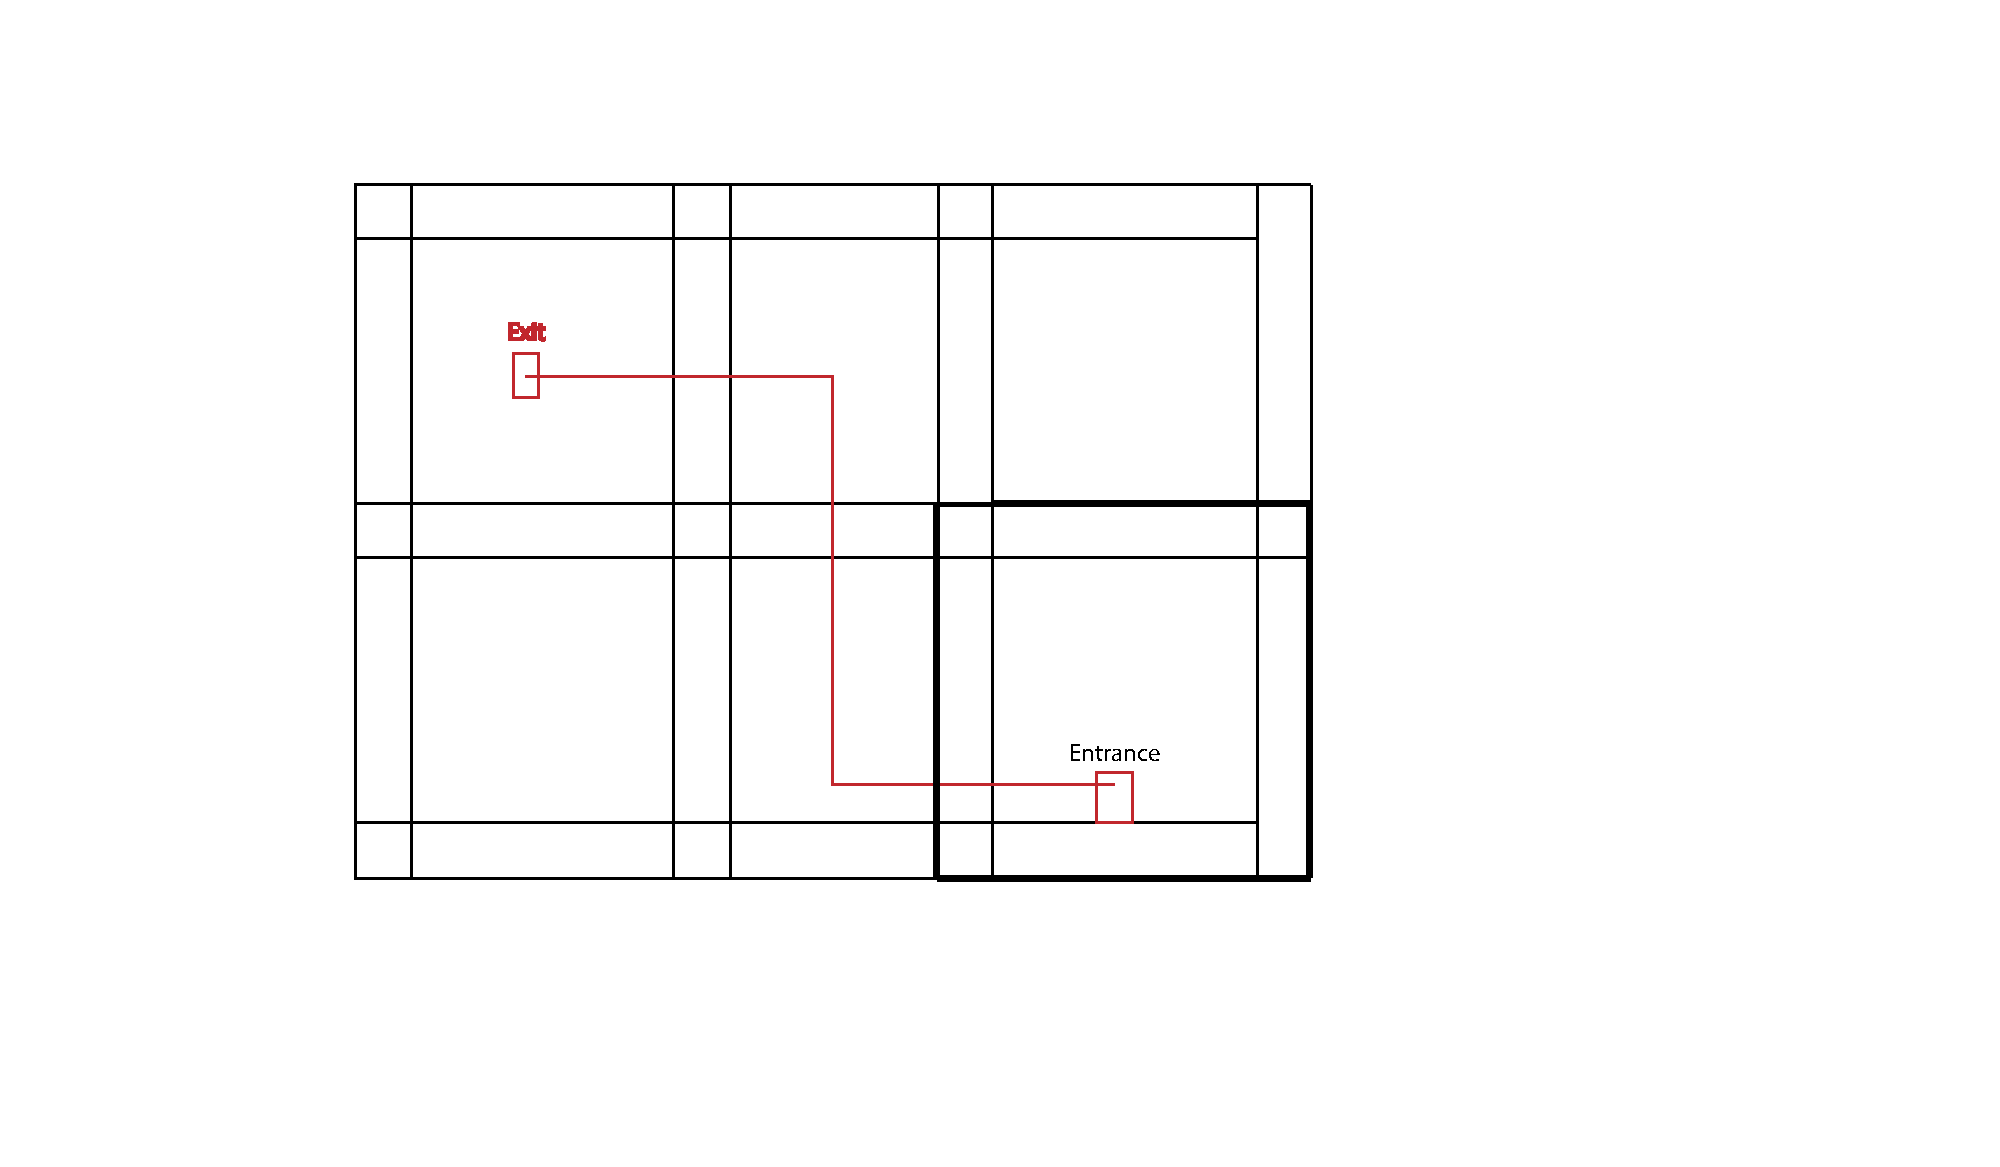
\includegraphics[scale=0.5]{Figures/Modules}
  \caption{Modules design. The lines represent where modules overlap.}
  \label{fig:Modules}
\end{figure}
\subsection*{Highscore \& Randomseed}
Using EEPROM we implemented two functions, $EEpromReadInt$ and $EEpromWriteInt$, which take use of the EEPROM library. These functions save unsigned integers to the EEPROM. They work by bitshifting the integer with 0 and 8 and then saving the two bitshifted values in the EEPROM. To extract from the board's EEPROM we grab the bitshifted values form their addresses in the EEPROM and then bitshift them with the respective number from before by using $EEpromWriteInt$. We add them together and then return the resulting integer.
\newline
We also use this for our random seeds that generate our level when the board is powered on. When the board is powered on we find the random seed on the address and apply it to the level generation. We then generate a new random unsigned integer and we save it on the same address for the next reboot.
\newline
The reason we need to recall the randomseed, is to ensure the game starts with a new seed each time the sketch is uploaded. If we don't provide the randomseed with a number, it will result in the exact same levels each time, making the level generator pointless. Now, we recall the old randomseed and use it to create a new randomseed, which is saved. This ensures that the map is different each time.

\section{Gameduino 2}
\subsection*{Graphics}
\subsubsection*{Rendering}
The Gameduino 2 consists of an essential graphics processing unit (GPU) with 256 kilobytes of RAM. With it is the ability to draw virtually anything on the screen. The way an object is drawn is through simple preparations before actually drawing it. The first step is call the Begin command from the Gameduino library with the type of object about to be drawn. Thereafter one has the option to make changes to the object before drawing it. 

\subsubsection*{Bitmaps}
 There is support for drawing images, called 'bitmaps'. With the exception of the background and text, everything the player witnesses in our game consists of these bitmaps. Since images are not uploaded along with the code to the Arduino, we store them on a microSD card which conveniently can be read in real time from the Gameduino 2. The simplest way to read a single image off the card would be to directly load it to the GPU with a command in the code. Each image loaded in would be assigned to a specific address and could thereafter be drawn with the image's top left corner at a given x-y coordinate. However, this method would not be able to fulfil the necessary requirements of what we had planned. This is where the Gameduino 2 asset converter comes in.

\subsubsection*{Assets}
The asset converter basically takes multiple media files, including images and sounds, and compiles them into a single asset file with the extension '.gd2'. As the abbreviation suggests, this file is specifically designed for the Gameduino 2 to read and gets placed on the SD card. Along with the asset file, a header file is generated to be included alongside the code in the associated project. The header file automatically defines constants associated with each image. There are four constants: handle, width, height, and cells. An image's handle is its index in the array of images provided, e.g., the first image would have the handle, 0. The width and height simply state the dimensions of the image in pixels. The 'cells' variable states how many images are included in the handle. Essentially we used handles with multiple cells (images) instead of a single image to easily maintain each animation. Here we can see the process of creating simple walking and attacking animations for our hero. Once the header file is included in a project, its constants are ready to be called from the code and used to project animations onto the screen.


\begin{figure}[h]
  \centering
  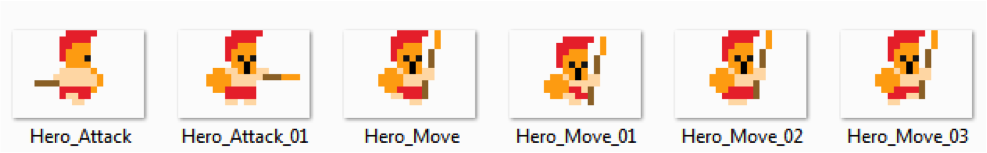
\includegraphics[scale=1]{Figures/HeroAttack}
  \caption{Hero attack sprites}
  \label{fig:Hero_Attak}
\end{figure}

\begin{figure}[h]
  \centering
  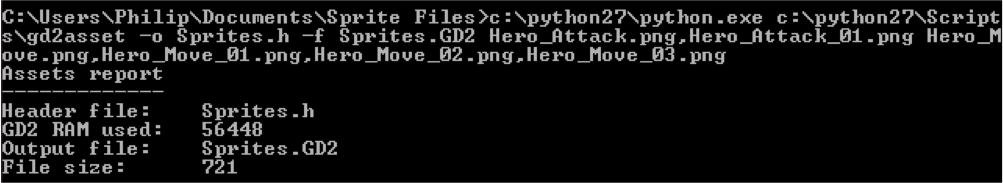
\includegraphics[scale=0.95]{Figures/Asset_cmd}
  \caption{Asset conversion in command line}
  \label{fig:asset_cmd}
\end{figure}


\begin{figure}[H]
\begin{minipage}[b]{0.45\linewidth}
  \centering
  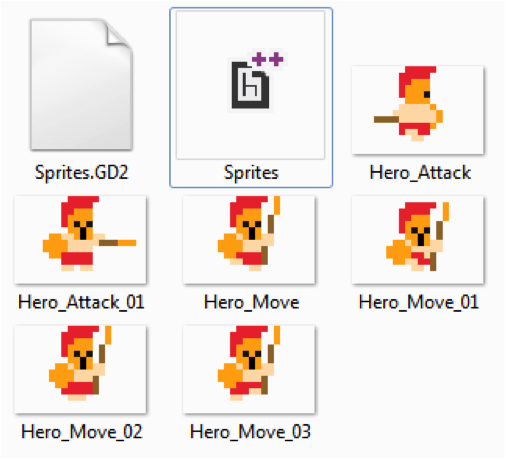
\includegraphics[scale=0.7]{Figures/Asset_output}
  \caption{The sprites and the output files}
  \label{fig:Asset_output}
\end{minipage}
\hspace{0.5cm}
\begin{minipage}[b]{0.45\linewidth}
  \centering
  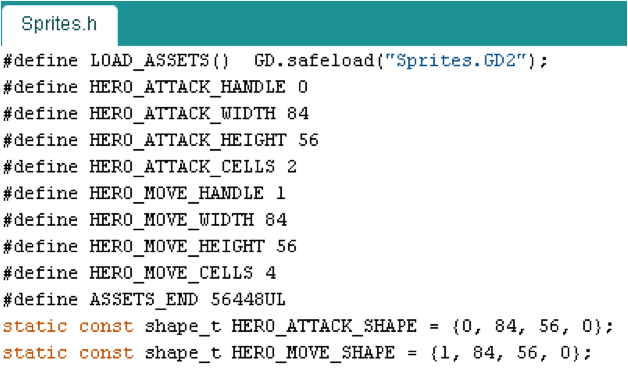
\includegraphics[scale=0.7]{Figures/SpritesHeader}
  \caption{The output from asset conversion}
  \label{fig:SpritesHeader}
\end{minipage}
\end{figure}

\newpage
\subsubsection*{Animation}
There are many ways to make sure an object in the game knows which handle it should use as well as which cell within the animation to display. The example in the Gameduino 2 reference utilizes both a sprite's x-coordinate and bit shifting as the object moves across the screen. This method however, is very primitive and specifically tailored to sprites moving from left to right. The way our program cycles through the cells of an animation is through time. \newline
Every object in the game that includes animation is a prop. That is to say the hero, minotaurs, and coins are all props. The prop class includes two functions directly related to animating: newHandle and updateAnimation. newHandle includes three parameters that get called from the specific object's class every update. It starts by checking if it should change anything about the animation by first checking if {\tt \_animLock} boolean is true. {\tt \_animLock} assures that the animation can't change until the current animation has gone through all its cells. We use this boolean when the hero attacks because he should finish an attack before reverting back to whichever movement animation he's in. The function also checks if the new handle or frame rate are the same as the current ones. If the conditions are met, the three values are replaced with those associated with a new animation and current cell to be displayed is manually set to the first one in the sequence.\newline
The function, updateAnimation, receives the parameter, dTime, from the main class every update. The {\tt \_dtime} variable keeps track of the number of milliseconds that have passed since the last update, or run-through of all the code. It is used to keep the time interval between cells consistent with the time it takes to update the whole program. Every animation has a manually set frame rate which determines how many milliseconds should pass before changing to the next cell. The variable, {\tt \_aniTime}, simply adds the value of {\tt \_dTime} to itself every update until the compiled number of milliseconds passed surpasses that of the animation's frame rate. When this happens, it is time to move on to the next cell in the animation. If however, it is the last cell, then it naturally reverts back to the first. One condition on resetting the cycle however that is that the {\tt \_aniStop} boolean is not used. This boolean is only used when an animation should not cycle back to its first cell. We use it primarily for death animations because when a unit dies it should stay dead. If the previously mentioned lock boolean is being used when a animation sequence resets, it is not required thereafter and set back to false. In any case, when a cell changes, the value of {\tt\_aniTime} is set back by the value of the animation’s frame rate so that it can once again accumulate time until it reaches the required frame rate value again for the next cell.

\subsubsection*{Drawing Sprites}
When the correct image to display is determined, there is still a matter of how to draw it and where exactly to place it. Rather than creating mirror image files we are able to use the Gameduino 2 functions to flip an image horizontally and still keep it at the same position. We intentionally made every sprite face to the right in the original images so we would only have to flip them if they are supposed to face left. As mentioned, everything that gets drawn with the Gameduino 2 gets prepared and manipulated beforehand. In this case, the image gets flipped, drawn, then flipped back again in case a sprite is updated thereafter to face to the right again. \newline


\begin{figure}[ht]
\begin{minipage}[b]{0.47\linewidth}
  \centering
  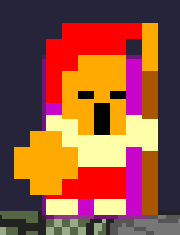
\includegraphics[scale=0.5]{Figures/herohitbox}
  \label{fig:herohitbox}
\end{minipage}
\hspace{0.5cm}
\begin{minipage}[b]{0.4\linewidth}
  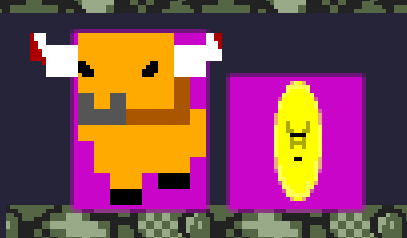
\includegraphics[scale=0.5]{Figures/minocoinhitbox}
  \label{fig:minocoinhitbox}
\end{minipage}
  \caption{The purple hitbox represents the body of the probs}
\end{figure}



In terms of coordinate placement, the image would under usual circumstances share the same position and dimensions as the hitbox it is registered to. However, our units have appendages/weapons/armor etc. which should not be included. Essentially we created sprites wherein the body of the characters is the same size as their respective hitbox and centered precisely in both the x and y axis on the whole image. It is also vital that all the images tailored to a specific object have the same dimensions. This is due to the way we coded where in respect to an object's hitbox the image should be drawn. Where each object includes specified hitbox dimensions, they also include image dimensions provided by the sprite header file. For each axis, the difference between half the image length and half the hitbox’s would be the distance between their centers if they were drawn at the same point. We simply subtract this value from the hitbox’s position in each axis respectfully and draw the image. Rather than sharing the same top left corner, the image and hitbox share centers.  When the image is always centered on the hitbox, it does not matter if the hitbox changes size. This system is useful when we want to implement ducking because as long as the ducking images have the body of the figure centered and the same dimensions as all the object’s other images, the image will translate accordingly.


\subsection*{Sound}
The Gameduino 2 requires the sound files to be converted using the asset converter. Before we include the sounds in the GD2 file, we need to convert them to an acceptable format. The assets converter only accepts files with following properties: 
''They need to be in .wav format, audio channel set to mono, and bit resolution set to 16.''

The conversion process also includes reducing the sample rate of the sound. By doing so,
the file will not take as much memory. Sometimes the sounds would get ruined by reducing too much,
so we had to find a balance between quality and size.


\section{Input}
Before implementing the nunchuk, we checked other alternatives. Both Arduino and the Gameduino 2 shield give us opportunities to control the game. Arduino can communicate with a PC and get data when a key is pressed on the keyboard. The Gameduino 2 is equipped with a touch screen and a accelerometer. We could have used one of these to get input, but none of them give a natural way to play a 'platformer' on a Gameduino 2. The PC solution does not feel natural as the keyboard and the Gameduino 2 screen usually are not in front of each other. The touch screen is not as responsive as we wanted and it would be hard to see the screen as the fingers will get in the way. The accelerometer is just wrong in all ways: it is hard to control, as you always has to 'guess' how to hold the device. The best option was using an external controller - a Wii nunhcuk.



\section{Optimization} %Cebrail / Carsten
Officially the \emph{flash memory} has a capacity of 32 Kb, but the IDE does not allow uploading sketches larger than 28.672 bytes. Furthermore, the first 4242 bytes are reserved for the \emph{bootloader}, so in reality we only have 24.430 bytes of code available. %Explain flash memory & bootloader?
\newline
Early optimizations is usually the bane of programming, but halfway through development we hit the code size ceiling. The code size seemed to arbitrarily grow independent of the code additions. From then on, every single addition required an optimization at least of same size, and in the end we had to sacrifice some maintainability and readability to reach our goals. Development stopped when optimization work yielded less than a 100 bytes per hour, but at that point the game was feature complete, so it just saved us from gold plating. Figure~\ref{fig:code_size} is a graph of the code size during development.
\newline
Arduino's IDE did not make it easy for us to optimize the game. All warnings concerning dead code or unused variables and functions are suppressed. Allegedly, the warnings were thought to discourage new developers, and was removed. The compiler was already optimized to removed these parts of the code, but it does so silently to the developer.
\newline
At one point we found that all the images we used combined exceeded the 256 KB RAM limit of the GPU. A quick solution was to simply format some of the images in a way that they took less space in the gd2 file. Luckily there was a format specifically designed for retro gaming sprites like ours, ARGB2. Manipulating an image with this bitmap pixel means that each variable in the red, green, blue, and alpha scheme contains two bits; alpha dealing with the opacity of a pixel.  Fortunately since our sprites do not consist of semi-transparent pixels or smooth edges, this format worked in our favor and significantly reduced the use of RAM.

\subsection*{Libraries} %Carsten / Cebrail
The external libraries use a lot of space. This is especially true for the Gameduino 2 library. It has been difficult to evaluate just how much space they use. For example, the difference in space between two and one function call, is the size of the call, but the difference between one and zero calls is the entire function plus the call. This is because the compiler cuts unused functions, and it makes it difficult to evaluate what parts of the code are expensive.
\newline
In any case, we could not do without the use of external libraries, nor would it be certain that we could rewrite them better. It would have taken too much time to optimize and test the libraries, and would probably not have been more profitable than optimizing our own code.

\subsection*{Verbosity} %Carsten
Maintainability is usually a great priority in programming, but the constraints of the Arduino left us to optimize for efficiency. In many cases the code was also left less readable and robust, in favor of using less space. There was, however, a certain limit where we did not simplify. For example, two versions of the same method return a random direction, either $-1$ or $1$:
\begin{verbatim}
char getRandDir() {
  if(random(2) == 0)
    return -1;
  else
    return 1;
}

char getRandDir() {
  return random(2) * 2 - 1;
}
\end{verbatim}
The first function is more expensive, but also a lot more readable. The second is absolutely incomprehensible, but cheaper. We went the top method, so the intent of the code was at least understandable. This case is more symbolic of the standard we held, since the top most function only cost 4 bytes more, but it serves as a good example. In the source code, the directions are replaced with the enumeration values {\tt LEFT} and {\tt RIGHT}. In other cases, for example the map generator, we split the code up in functions for readability.

\subsubsection*{Encapsulation} %Cebrail / Carsten
Usually it is good code practice to encapsulate variables and use getters and setters. This was a luxury we could not afford, which became apparent when we hit the ceiling. Most variables was made public, though in some cases a getter was cheaper than directly accessing the variable.

%Too obvious?
%\subsubsection{Repeated statements} %Cebrail
%Repeated statements - well it speaks for itself. Repeating something that has been calculated before is just a waste of code space. Simplifying the code in this manner is sometimes not easy, it requires that you think creative. It often requires you to think - is this needed? It may not always be obvious. Often it is about finding a shortcut to some calculation and taking advantage of already existing results.


\subsection*{Datatypes} %Cebrail
A good place to start was the datatypes. Converting the bigger datatypes to some smaller ones was an easy optimization. Mostly, it was integers that were converted to data types like {\tt char}, {\tt byte} and {\tt word}. {\tt char} is capable of encoding numbers from -128 to 127. While {\tt bytes} is a 8-bit unsigned number, from 0 to 255 and {\tt word} is basically an unsigned 16-bit number, from 0 to 65535. Notice that {\tt byte} is the unsigned version of {\tt char}. More details are found on Arduino's site\footnote{http://arduino.cc/en/Reference/HomePage}.

\subsection*{Global Variables} %Carsten
Like Java's main function, Arduino has two special functions: {\tt setup} and {\tt loop}. The former is called once on program start, while the latter is repeatably called until the Arduino is turned off.\footnote{At least, we haven't discovered a way to terminate a sketch.} This is not a very optimized structure. It forces us to use global variables if we want to reuse anything from setup in loop. Our solution was to leave {\tt loop} empty and put an endless loop in {\tt setup} instead. All of our variables could become local with this change, greatly reducing code size.

\subsection*{Inconsistencies} %Carsten
Finally, in some cases the code size arbitrarily increased or decreased where it should not have. For example, there are some unused values in the {\tt Sprite.h}, which was generated by the asset converter. If these are removed, the code size increases. This is probably some inconsistency in the compiler, but we did not research this further. In other cases, where more code resulted in less code size, we removed the anomalies (or simply did not add them), but the asset converter values was discovered when space was really limited, so we had to leave it in.
